\section{Ontologie} \label{ontologies}
Všechny jazyky pro reprezentaci znalostí, které nejsou založeny na logice mají své nedostatky. Nejčastěji je problém v nedostatku sémantiky. Logika těmto jazykům potřebnou sémantiku dodala a můžeme jí díky tomu prohlásit za nejpřesnější způsob, jak znalosti formálně reprezentovat. (ne nutně nejefektivnější)\par
V této sekci přejdeme od konkrétních jazyků ke komplexnějšímu pohledu na reprezentaci znalostí. Ontologie lze také považovat za formální jazyk reprezentace znalostí. Jsou  však spíše realizací předchozích formálních jazyků než-li nový teoretický pohled na reprezentaci znalostí.\par
\subsection{Význam a Definice}
Význam slova ve filozofii odkazuje na tzv. "jsoucno", tedy zkoumání existence. Se zkoumáním existence úzce souvisí otázka: \textit{Co existuje?}. K odpovědi na tuto otázku je nutný systematický postup. Potřebujeme definovat tzv. ontologické kategorie, do kterých všechny zkoumané objekty rozdělíme. Příkladem takových ontologických kategorií mohou být: \textit{lidé, zvířata, věci}. Konkrétní existující instance 
% (nazveme je \textit{individuality} jako v případě předchozích formálních jazyků) 
jsou potom např. \textit{člověk Jiří, pes Alík, česká královská koruna}. Přesně z této ideje ontologických kategorií vychází význam slova ontologie v počítačových vědách. \cite{Stephan2007} Nejedná se tedy o stejné zkoumání jako v případě filosofie, ale stále se pohybujeme ve stejné oblasti.\par
Ontologickými kategoriemi obecně určujeme, které znalosti budeme schopni reprezentovat - určujeme specifickou doménu, pro kterou znalosti modelujeme. Tvoříme tak tzv. \textit{ontologický slovník}.\par
% Zde je možné najít souvislost s ostatními formálními jazyky - ontologie v podstatě popisují názvy hran v sémantických sítích, popř. logické vzorce, používané pro reprezentaci znalostí.\cite{Stephan2007}\par
Obecně ontologie tedy popisují, co v dané doméně existuje. Ontologie jako konkrétní počítačový artefakt (např. soubor) kóduje danou znalost o doméně v počítačem zpracovatelné formě.\cite{Stephan2007}\par
\noindent Doslovná definice ontologie dle \cite{gruber1993translation} je:\par
\begin{quote}
    \textit{Ontologie je explicitní specifikace konceptualizace.}
\end{quote}\par
\noindent Později byla tato definice rozšířena dle \cite{Borst97} na:\par
\begin{quote}
    \textit{Ontologie je formální specifikace sdílené konceptualizace.}
\end{quote}\par
\subsection{Základní charakteristiky}
\begin{enumerate}
\item Formální
\begin{itemize}
\item Ontologie musí být vyjádřena formálním jazykem (výhody těchto jazyků jsou popsány v kapitole č. \ref{sec:terms} sekce č. \ref{sec:jazyk}).
\end{itemize}
\item Explicitní
\begin{itemize}
\item Znalost musí být vyjádřena maximálně explicitně, pro optimální strojové zpracování.
\end{itemize}
\item Sdílené
\begin{itemize}
\item Ontologie vždy reflektuje dohodu skupiny lidí v dané doméně, v podstatě se jedná o kolektivní ontologické závazky (viz sekce č. \ref{ontological_commitments}).
\end{itemize}
\item Konceptuální
\begin{itemize}
\item Ontologie popisuje znalosti pomocí symbolů, které reprezentují koncepty a relace mezi nimi. Konceptualita spočívá v tom, že jsou ontologie intuitivně uchopitelné pro člověka, protože odpovídají lidskému mentálnímu modelu znalostí. Jako protipříklad lze uvést neuronové sítě, které též reprezentují určité znalosti, ale přirozenému lidskému chápání je to již vzdáleno.
\end{itemize}
\item Doménově specifická
\begin{itemize}
\item Ontologie je vždy omezena na určitou oblast - doménu.\cite{Stephan2007}
\end{itemize}
\end{enumerate}

% Ontologie jsou v praxi používány v informačních systémech pro rozhodování a vyvozování (angl. reasoning) v dané doméně.\cite{Stephan2007}\par

\subsection{Základní stavební kameny}
\begin{itemize}
\item Koncepty
\begin{itemize}
\item V sémantických sítích i v deksripční logice se tento konstrukt nazývá stejně
\item Reprezentují ontologické kategorie
% \item V příloze na obrázku č. \ref{fig:ontology_example} např. City
\end{itemize}
\item Relace
\begin{itemize}
\item Analogicky se jedná o hrany sémantické sítě nebo role v deskripční logice
\item Propojují koncepty a instance - reprezentují vazby mezi nimi
% \item V příloze na č. \ref{fig:ontology_example} např. locatedIn
\end{itemize}
\item Instance
\begin{itemize}
\item Individuality v sémantické síti nebo v deskripční logice
\item Reprezentují konkrétní objekty v doméně \cite{Stephan2007}
% \item V příloze na obrázku č. \ref{fig:ontology_example} např. Berlin
\end{itemize}
\end{itemize}
%Ontologii si lze také představit jako množinu výroků (axiomů) např. \textit{OsobaX je člověk} apod.  \cite{Stephan2007}\par
\subsection{Zápis ontologií}
Ontologie lze zapisovat několika způsoby. Například pomocí sémantických sítí, které typicky neobsahují všechny důležité informace, jelikož nejsou tak expresivní (viz sekce č. \ref{fig:semantic_network}). Toto zobrazení je příznivé hlavně pro pochopení lidmi. Dále je zapisujeme pomocí serializovaného formátu (např. XML), vhodného pro strojové zpracování. Dále pomocí logických vzorců, to je vhodné pro další vyvozování (angl. reasoning). \cite{Stephan2007}.

\subsection{Použití ontologií}
\begin{itemize}
\item \textbf{Propojení znalostí} - jednotný znalostní slovník napříč aplikacemi, datový zdroj znalostí
\item \textbf{Abstrakce znalostí} - zdroj schématu znalostí (hierarchie a vztahy konceptů) pro budoucí využití
\item \textbf{Automatizace zpracování znalostí} - automatické vyvozování závěrů z platných axiomů (angl. reasoning)
\item \textbf{Integrace informací} - integrace na úrovni různých datových schémat a interpretace získaných dat z jednoho zdroje v rozdílném schématu
\item \textbf{Získávání informací} - zdokonalování modelu znalostí s důrazem na jeho prohledávání
\item \textbf{Sémantická správa obsahu} - přidávání metadat k datům, která později slouží k jejich lepší identifikaci a lepšímu přístupu k nim
\item \textbf{Organizace znalostí} - sdílený znalostní model daného seskupení lidí (např. firma, škola)
\item \textbf{Expertní systémy} - systémy schopné řešit komplikované otázky (úlohy) - např. i v medicíně \cite{Stephan2007}
\end{itemize}
\subsection{Typy ontologií}
Existují čtyři základní typy ontologií. Jednotlivé typy se od sebe liší úrovní abstrakce reprezentovaných znalostí. \cite{Stephan2007}\par
\begin{itemize}
\item \textbf{Top-level}
\begin{itemize}
\item Abstraktní a obecné koncepty (např. \textit{fyzický objekt, abstraktní objekt}) s velkým potenciálem znovupoužití v mnoha doménách
% \item typicky se přímo nenachází v aplikacích - spíše ontologie, které se jimi řídí
\item Typicky se používají jako předloha pro tvorbu ontologií zmíněných níže
\item Příklady UFO \cite{Guizzardi2005}, SUMO \cite{Niles:2001:TSU:505168.505170}, DOLCE \cite{Dolce}
\end{itemize}
\item \textbf{Doménové a úkolové ontologie}
\begin{itemize}
\item Zachytávají znalost ve specifické doméně - např. medicíně, geografii; nebo znalost o specifickém úkolu - např. diagnostika, konfigurace
% \item Doménové ontologie se zaměřují na "statické" znalosti o doméně, úkolové potom na postupy, plánování, monitoring apod. - "dynamické" znalosti
\end{itemize}
\item \textbf{Aplikační ontologie}
\begin{itemize}
\item Propojují doménové a úkolové ontologie pro účely konkrétní aplikace
\end{itemize}
\end{itemize}
Jedná se o inkluzivní hierarchii, nižší ontologie přejímají a konkretizují obecné koncepty a relace vyšších ontologií. \cite{Stephan2007}
\begin{figure}[htbp!]
	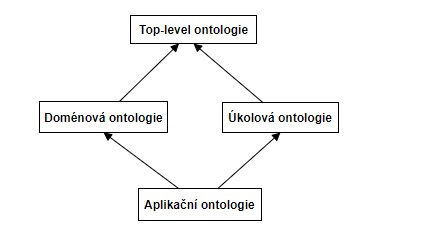
\includegraphics[width=0.7\linewidth]{img/ontology_types.png}
	\caption{Typy ontologií (zdroj \cite{Stephan2007}, přeložil autor)}
	\label{fig:ontology_types}
\end{figure}


\subsection{Přidružené technologie, standardy a další}
% Existuje několik jazyků, které jsou určené pro zápis a jednoznačnou reprezentaci ontologií ve strojově čitelné formě. Uvedeny jsou pouze ti nejpoužívanější kandidáti.
\subsubsection{RDF}
V doslovném překladu se jedná o framework pro popis zdrojů. RDF je standardizovaný jazyk pro reprezentaci znalostí (informací) na webu. Tento jazyk lze však použít pro reprezentaci libovolných znalostí.\par
\paragraph{Základními elementy jsou:}
\begin{itemize}
\item URI (Uniformní identifikátor zdroje) - slouží k pojmenování a identifikaci individualit, konceptů a jejich vlastností (příklad je \textit{urn:isbn:0451450523}, což je URI knihy)
\item Věty ve tvaru: \fbox{Podmět} $\xrightarrow{\text{\textit{Predikát}}}$ \fbox{Předmět} (jednotlivé členy jsou ve tvaru URI)
% \begin{itemize}
% \item []\textbf{Příklad} \fbox{http://web.de/MrX.html}$\xrightarrow{\text{\textit{btr:maAutora}}}$ \fbox{btr:PanX} \cite{Stephan2007}
% \end{itemize}
\end{itemize}
RDF je typicky zpracováváno v serializované podobě v XML formátu (viz příklad níže) \cite{Stephan2007}. Poměrně populární variantou pro serializaci RDF je též JSON-LD \cite{JSON_LD} nebo Turtle \cite{TURTLE}.\par

\begin{lstlisting}[caption= Příklad syntaxe RDF XML, captionpos=b]
<rdf:Description rdf:about="http://ubiqbiz.com/web/MrX.html">
    <btr:hasAuthor rdf:resource="btr:PanX"/>
</rdf:Description>
<rdf:Description rdf:about="btr:PanX">
    <btr:employedAt rdf:resource="btr:UbiqBiz"/>
</rdf:Description>
\end{lstlisting} 

RDF je framework pro prostý popis zdrojů, pokud chceme datům dávat význam a s tímto významem pracovat, musíme využít další rozšíření. Typicky datům dodáváme soubor axiomů pro další vyvozování (angl. inference) popř. uvažování (angl. reasoning), které nám umožní je dále rozvíjet a efektivně s nimi pracovat. V následujícím seznamu uvádíme příklady takových rozšíření.
\begin{itemize}
\item Vyvozování dalších znalostí, popis schématu
\begin{itemize}
\item \textbf{RDFS} - omezené prostředky na rozdíl od pokročilejších \par(zdroj: \url{https://www.w3.org/TR/rdf-schema/})
\item \textbf{OWL} - ve své podstatě univerzální jazyk pro popis ontologií \par(zdroj: \url{https://www.w3.org/TR/owl2-primer/}, podrobněji níže)
\end{itemize}
\item Validace modelu
\begin{itemize}
\item \textbf{SHACL} - validace RDFS (zdroj: \url{https://www.w3.org/TR/shacl/})
\end{itemize}
\end{itemize}

\subsubsection{SPARQL}
\noindent Dotazovací jazyk standardizovaný pro vyhledávání a další operace v RDF \cite{SPARQL}.\par
\subsubsection{OWL}
\noindent Web Ontology Language (OWL) je  standardizovaným jazykem pro sémantickou anotaci webového obsahu. Jazyk má 3 varianty, my se zaměříme pouze na nejčastěji používanou a to je OWL-DL (z angl. \textit{OWL description logic}).\par
Syntaxe OWL zakládá na RDF a rozšiřuje jej. Větám (trojicím) dává ve své podstatě další sémantiku, kterou lze později interpretovat.\par
% \paragraph{Základními konstrukty jsou:}
% \begin{itemize}
% \item Třídy (koncepty z DL)
% \item Vlastnosti (role z DL)
% \item Individuality (v DL stejně)
% \item Konstruktory tříd (slouží k tvorbě složitějších tříd)
% \end{itemize}
Dokument v jazyce OWL je v podstatě množina výroků, které mohou být interpretovány jako axiomy v deskripční logice. OWL je mocný nástroj, jelikož vychází z deskripční logiky a převzalo její výhody - je možné kontrolovat konzistenci a vyvozovat implicitní znalosti. \cite{Stephan2007}

\subsubsection{OntoUML}
Rozšíření jazyka UML určené pro modelování ontologií. Toto rozšíření je založeno na top-level ontologii UFO \cite{Guizzardi2005}.

\subsubsection{SKOS}
SKOS (z angl. Simple knowledge organization system) je standard pro sdílení strojově čitelných dat. Tento standard řeší základní problém systémů pro organizaci znalostí (zkratka KOS). Tyto systémy operují se znalostmi v různé formě~-~např. obecné slovníky, thesauri, taxonomie, klasifikační schémata. SKOS standardizoval sdílení těchto dat v jednotné formě, která zachovává výhody původních forem (slovníky, thesauri...). Cílem je mít data dostupná v jednotném formátu - RDF. \cite{SKOS}\par 
% OWL Full ontologie \cite{OWL_FULL}.
Standard SKOS klade menší důraz na formálnost, míří více na přímou konverzi dat na znalosti a jejich použití v různých situacích. Neklade takový důraz na uvažování (angl. reasoning) a vysokou přesnost dat. \cite{isaac2009skos}\par 
SKOS je ve své podstatě ontologií, jak je možné vidět na obrázku v příloze \ref{fig:SKOS-ontology}. 

% Bližší specifikace SKOS je dostupná zde https://www.w3.org/TR/2005/WD-swbp-skos-core-guide-20051102/#secabout.\cite{SKOS}

%TODO příklad OWL












